\section{GIR-Enabled Two-Level Parallel Execution}
\label{sec:task_parallel}



% Fortunately, GIR eliminates this barrier because we persistently store the graph's structural decomposition, including WCCs at the connectivity level, SCCs and their condensation DAG at the cycle level, and BiCC blocks and the BC tree at the biconnectivity level.
% These components are always available without recomputation.
% With that, given a query, GIR first uses its three-level hierarchy to immediately identify a set of structurally independent blocks.
% Then, GIR assigns each block as an independent task, and executes all tasks concurrently.
% Further, within each task, conventional data parallelism processes the local subgraph.
% To this end, it creates a \textit{\textbf{two-level parallelism model, i.e., task parallelism across blocks, and data parallelism within each block}}.





% The speedup scales not only with the number of vertices per block, but also with the number of independent blocks in scope.



%figures insertion,
%technology all done



\subsection{The Two-Level Parallel Execution Model}
\label{subsec:framework}

Most parallel graph computation frameworks rely on \textit{data parallelism}~\cite{Shun2013Ligra,Wang2016Gunrock,Zhang2018GraphIt}. That is, they process one task with many vertices or edges simultaneously using all the available threads (or cores).
This approach leaves a second, orthogonal source of parallelism unexploited, i.e., 
\textit{task parallelism}, where structurally independent subgraphs execute as concurrent tasks.
% This approach leaves a second, orthogonal source of parallelism unexploited, i.e., \textit{task parallelism},
% where structurally independent subgraphs execute as concurrent tasks.
It is difficult to achieve on flat graph representations because structural boundaries are not explicitly stored and must be recomputed from scratch at each query.

Fortunately, GIR eliminates this barrier by persistently maintaining the graph's three-level structural decomposition.
Motivated by this opportunity, we design a \textit{{two-level parallelism model, i.e., task parallelism across blocks, and data parallelism within each block}}.
In the following, we first discuss the theoretical foundation for this model and then apply it to BFS and other algorithms.


% We establish the structural properties of GIR that enable independent task execution,
% then define the class of algorithms that exploit them.

% \textbf{Notation.}
Let $G = (V, E)$ be a directed graph.
GIR maintains a three-level structural hierarchy.
At the WCC level, GIR stores  $\{W_1, \ldots, W_p\}$.
At the SCC level, GIR stores $\{C_1, \ldots, C_q\}$
and their condensation DAG $\mathcal{D} = (\mathcal{V}_{\mathcal{D}}, \mathcal{E}_{\mathcal{D}})$.
At the BiCC level, for each SCC $C_k$,
GIR stores the BiCC blocks $\{B_1^k, \ldots, B_{r_k}^k\}$
of the underlying undirected graph $\hat{G}[C_k]$,
organized as a BC tree $\mathcal{T}_k$.
A vertex $a$ is an \textit{articulation point} of $C_k$
if its removal from $\hat{G}[C_k]$ increases the number of connected components.
We write $\partial B$ for the set of articulation points on the boundary of block $B$.
We write $G[B]$ for the subgraph of $G$ induced by the vertices of $B$.

These three levels provide three distinct structural boundaries at which
computation can be partitioned. We formalize each with a separation lemma.

\begin{lemma}[WCC separation]
\label{lemma:wcc_sep}
Let $W_i$ and $W_j$ be two distinct WCCs of $G$.
No path exists between any vertex in $W_i$ and any vertex in $W_j$.
Any algorithm whose output for a vertex $v$ depends only on vertices
reachable from $v$ is fully independent across WCC boundaries.
\end{lemma}

\begin{lemma}[SCC-DAG separation]
\label{lemma:scc_sep}
Let $C_i$ and $C_j$ be two SCCs such that $C_j$ is not reachable from $C_i$
in the condensation DAG $\mathcal{D}$.
No directed path exists from any vertex in $C_i$ to any vertex in $C_j$.
Any algorithm whose output for vertices in $C_i$ depends only on vertices
reachable from $C_i$ is independent of $C_j$.
\end{lemma}


\begin{lemma}[AP separation]
\label{lemma:ap_sep}
Let $B_i$ and $B_j$ be two distinct BiCC blocks within the same SCC $C_k$,
with $u \in B_i$ and $v \in B_j$.
In graph $\hat{G}[C_k]$,
every path between $u$ and $v$ passes through every AP
on the unique path between $B_i$ and $B_j$ in the BC tree $\mathcal{T}_k$.
Consequently, the distance $d(u, v) = d(u, a^*) + d(a^*, v)$
for any AP $a^*$ on the BC tree path from $B_i$ to $B_j$.
Since every directed edge in $G[C_k]$ is also an undirected edge in $\hat{G}[C_k]$,
every directed path between $u$ and $v$ is also an undirected walk,
and therefore passes through every AP on the BC tree path.
Hence the distance decomposition extends to directed shortest-path distances as well.
\end{lemma}

\begin{proof}

\textit{Lemmas~\ref{lemma:wcc_sep} and~\ref{lemma:scc_sep} follow directly from
the definitions of WCCs and SCCs.
Lemma~\ref{lemma:ap_sep} follows from the definition of biconnected components.}
% \vspace{-1mm}
% and is a standard result in graph theory~\cite{tarjan1972depth}.} 
\end{proof}

Together, these three lemmas establish that GIR's three-level hierarchy
provides three provably independent partitions of the graph.
We now define which structural level is the right partition boundary
for a given algorithm.

\begin{definition}[Dependency level]
\label{def:dep_level}
The \textit{dependency level} of an algorithm $\mathcal{A}$,
written $\mathcal{L}(\mathcal{A})$$\in$$\{\textit{WCC}, \textit{SCC}, \textit{BiCC}\}$,
is the coarsest level at which $\mathcal{A}$'s computation
on a structural unit $S$ is self-contained given boundary values at $\partial S$.
\end{definition}

For example, a connected component labeling algorithm has
$\mathcal{L}(\mathcal{A}) = \textit{WCC}$ as
each component is fully independent with no boundary values.
A reachability query from a source $s$ has $\mathcal{L}(\mathcal{A}) = \textit{SCC}$ because only SCCs reachable from $C_s$ in $\mathcal{D}$ participate.
A shortest path algorithm has $\mathcal{L}(\mathcal{A}) = \textit{BiCC}$ because shortest paths between blocks
decompose exactly at APs based on Lemma~\ref{lemma:ap_sep}.

% We now define the class of algorithms that can exploit GIR.

\begin{definition}[Boundary-decomposable algorithm]
\label{def:boundary_decomp}
An algorithm $\mathcal{A}$ with dependency level $\mathcal{L}(\mathcal{A})$ is
\textit{boundary-decomposable} if it satisfies two conditions.
\begin{itemize}[leftmargin=*]
  \item \textbf{Local decomposability.}
    For each structural unit $S$ at level $\mathcal{L}(\mathcal{A})$,
    there exists a function $f_S$ such that
    $\mathcal{A}(v) = f_S\bigl(v,\; \lambda(\partial S),\; G[S]\bigr)$
    for all $v \in S$,
    where $\lambda(a)$ is the externally provided boundary value at $a \in \partial S$.
  \item \textbf{Boundary composability.}
    The global output of $\mathcal{A}$ can be assembled by propagating
    $\lambda$ values across structural boundaries in a single pass.
\end{itemize}
\end{definition}

\textit{Local decomposability} means the computation inside unit $S$ requires
no information from outside $S$ beyond the values at its boundary.
\textit{Boundary composability} means the global result follows from combining local results
at boundaries without a second global pass.
We now state the main result.

\begin{theorem}[Two-level parallel execution]
\label{thm:two_level}
Let $\mathcal{A}$ be a boundary-decomposable algorithm with dependency level
$\mathcal{L}(\mathcal{A})$.
GIR executes $\mathcal{A}$ correctly in two levels:
\begin{itemize}[leftmargin=*]
  \item \textbf{Level 1 (structural partitioning).}
    GIR identifies all structural units $\{S_1, \ldots, S_k\}$ at level $\mathcal{L}(\mathcal{A})$
    that are relevant to the query, using the separation lemma at that level.
    Irrelevant units are discarded without affecting correctness.
  \item \textbf{Level 2 (independent task execution).}
    GIR assigns each relevant unit $S_i$ as one independent task
    and executes all $k$ tasks concurrently.
    For each task, GIR provides boundary values $\lambda(\partial S_i)$
    before execution.
    After all tasks complete, GIR assembles global result
    via boundary composability.
\end{itemize}
The parallel execution time of Level 2 is
$\mathcal{O}\!\left(\max_{i}\, T(S_i)\right)$,
where $T(S_i)$ is the sequential execution time of $\mathcal{A}$ on unit $S_i$.
This compares to $\mathcal{O}\!\left(\sum_{i}\, T(S_i)\right)$ for sequential execution.
The task parallel speedup scales with $k$, the number of relevant structural units.
\end{theorem}

\begin{proof}[Proof]
\textit{Correctness.}
By the separation lemma at level $\mathcal{L}(\mathcal{A})$,
all information that crosses boundary of unit $S_i$ passes through $\partial S_i$.
Before Level 2 begins, GIR computes $\lambda(\partial S_i)$ for all $i$
via the structural traversal in Level 1.
By local decomposability, each task $S_i$ computes its correct local output
using only $G[S_i]$ and $\lambda(\partial S_i)$.
By boundary composability, combining local outputs at boundaries
produces the globally correct result.

\textit{Independence.}
WCCs and SCCs each partition $V$, so tasks at these levels share no vertices.
At the BiCC level, blocks partition the \emph{edges} of $G$, not the vertices.
That is, APs are shared across adjacent blocks,
but they appear only as read-only boundary values $\lambda(\partial S_i)$
that are fixed before Level 2 begins.
All non-boundary internal vertices belong to exactly one block.
Since no two tasks share any internal vertex or write to any shared state,
their executions do not interfere.
Tasks require no synchronization during Level 2.

\textit{Parallel time bound.}
Since all $k$ tasks are independent and execute concurrently,
the parallel execution time is determined by the slowest task. The speedup of this execution model over a flat-graph method grows with $k$.
\end{proof}

% The speedup of the two-level parallel execution model over a regular graph approach grows with $k$.
% For graphs with many small, tightly interconnected components,
% $k$ is large and speedup is substantial.
% For graphs dominated by a single large structural unit,
% the model degrades gracefully to standard data parallelism within that unit.



\subsection{Applications of the Two-Level Parallel Executation Model}
\label{subsec:instantiations}


We demonstrate the two-level parallel execution model on three algorithm families, i.e., graph traversal, path finding, and centrality.
For each, we identify its dependency level per Definition~\ref{def:dep_level},
verify that it is boundary-decomposable per Definition~\ref{def:boundary_decomp},
and describe how Theorem~\ref{thm:two_level} applies.
We use BFS as the primary concrete example.
% because its four-stage pipeline illustrates the framework in full detail.

\textbf{BFS and graph traversal.}
BFS is applied hierarchically across two structural levels.
At the SCC level ($\mathcal{L} = \textit{SCC}$), the output for any vertex $v$
depends only on vertices reachable from the source $s$ in $G$,
and reachability is SCC-bounded by Lemma~\ref{lemma:scc_sep}, while unreachable SCCs are pruned entirely.
Within each retained SCC, computation further decomposes at the BiCC level
($\mathcal{L} = \textit{BiCC}$).
By Lemma~\ref{lemma:ap_sep}, the BFS level of any vertex $v\in B$
equals to the entry level $\lambda(a^*)$ at $B$'s entry AP $a^*$
plus the local BFS level of $v$ within $B$.
This satisfies local decomposability with
$f_B(v, \lambda(\partial B), G[B]) = \lambda(a^*) + \ell_\text{local}(v, B)$.
Global BFS levels assemble by propagating entry levels across the BC tree,
satisfying boundary composability.
BFS is thus boundary-decomposable and Theorem~\ref{thm:two_level} applies.

Given a source $s$, GIR executes BFS in four concrete stages.

\textit{Stage 1: SCC pruning via the condensation DAG.}
GIR traverses $\mathcal{D}$ from the SCC $C_s$ containing $s$
and retains only the reachable set
$\mathcal{R} = \{C \in \mathcal{V}_{\mathcal{D}} : C_s \rightsquigarrow C\}$.
All SCCs outside $\mathcal{R}$ are provably irrelevant by Lemma~\ref{lemma:scc_sep}.
The time complexity of this stage is $\mathcal{O}(|\mathcal{V}_{\mathcal{D}}| + |\mathcal{E}_{\mathcal{D}}|)$.

\begin{figure}[t]
    \centering
    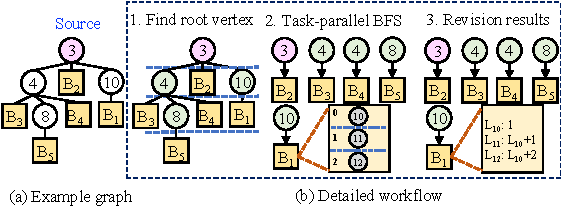
\includegraphics[width=1\linewidth]{figures/concurrent_bfs-crop.pdf}
    \caption{Concurrent BFS on GIR from root vertex 3. (a) shows an example graph in BC tree. (b) shows the BFS computation workflow.}
    \Description{Diagram of an example graph organized as a BC tree, and the four-stage concurrent BFS workflow that prunes SCCs, decomposes into block tasks, runs BFS per block, and merges global levels.}
    % The three-stage workflow: find block entry APs, run concurrent BFS per block, and assemble global levels.
    % \YJ{TODO, L10: 1}

    \label{fig:concurrent_bfs}
\end{figure}

\textit{Stage 2: Task decomposition via the BC tree.}
Within each retained SCC, GIR traverses the BC tree $\mathcal{T}_k$
in BFS order starting from the block $B_s$ containing $s$,
to identify the set of reachable blocks $\mathcal{B}_s$.
For the example graph in Figure~\ref{fig:concurrent_bfs}(a), starting form root vertex 3, $B_1$-$B_5$ are identified as reachable.
During this traversal, GIR computes the entry BFS level $\lambda(a_i^*)$
for each block $B_i \in \mathcal{B}_s$ in topological order along $\mathcal{T}_k$.
That is, the entry level of $B_s$ itself is 0, and the entry level of each subsequent block
is determined from 
% the already-computed level of 
its parent's entry AP.
Particularly, for the example graph, the entry levels of $B_1, B_2, B_3, B_4$, and $B_5$ are 1, 0, 1, 1, 2, respectively. 
This sequential pre-computation has time complexity $\mathcal{O}(|\mathcal{B}_s|)$.
Each block then becomes one independent task with all boundary values fixed.
By Lemma~\ref{lemma:ap_sep}, blocks share no internal vertices
and communicate only through APs.
Thus, all tasks in $\mathcal{B}_s$ are mutually independent once Stage 2 completes. 
% For the example graph in Figure~\ref{fig:concurrent_bfs}(a), source vertex 3 is in B2, and Stage 2 computes entry AP levels of 4 for B3, 8 for B4 and B5 (via vertex 4), and 10 for B1 (via vertex 8).

% \CQ{In Figure~\ref{fig:concurrent_bfs}, source vertex 3 is in B2, and Stage 2 computes entry AP levels of 4 for B3, 8 for B4 and B5 (via vertex 4), and 10 for B1 (via vertex 8).}
%\YJ{Figure example.}


\textit{Stage 3: Concurrent BFS within each block.}
GIR executes all $|\mathcal{B}_s|$ tasks concurrently.
Each task runs BFS from its entry AP $a_i^*$,
computing local BFS levels $\ell_\text{local}(v, B_i)$ for all $v \in B_i$.
Tasks require no synchronization during execution
and are assigned to independent CPU worker threads,
with all threads running simultaneously.
The parallel time complexity of this stage is
$\mathcal{O}\!\left(\max_{B_i \in \mathcal{B}_s}(|V_{B_i}| + |E_{B_i}|)\right)$.
For the five blocks shown in Figure~\ref{fig:concurrent_bfs}(b), they can run simutaneously.
% shows five blocks running concurrently. 
% \CQ{For example, B1's task runs BFS from entry AP vertex 10, computing local levels 0, 1, 2 for vertex 10, 11, 12 respectively, with no coordination needed from the other four tasks.}
% \YJ{TODO}

\textit{Stage 4: Global level revision.}
GIR revises the global BFS levels via boundary composability.
For each vertex $v \in B_i$, the global level is
$\ell(v) = \lambda(a_i^*) + \ell_\text{local}(v, B_i)$.
This merge is embarrassingly parallel and requires no further traversal. 
% \CQ{Continuing the B1 example, vertex 10 has $\lambda(a^*) = 2$ and local levels 0, 1, 2, so global levels are $L_{10}{=}2$, $L_{11}{=}3$, $L_{12}{=}4$.}
For block $B_1$ in Figure~\ref{fig:concurrent_bfs}(b), the global BFS level of each vertex becomes the sum of its local level plus 10's level.

% The same task decomposition applies to DFS, providing a practical path to parallelizing a traditionally sequential primitive.
% \YJ{Figure example.}


\textbf{Path finding.}
SSSP and $k$-shortest paths (KSP) have dependency level $\mathcal{L} = \textit{BiCC}$.
By Lemma~\ref{lemma:ap_sep}, every path between $u \in B_i$ and $v \in B_j$
passes through the AP $a^*$ between them.
Therefore $d(s, v) = d(s, a^*) + d_\text{local}(a^*, v, B_j)$,
where $d_\text{local}$ is the shortest-path distance within block $B_j$.
This satisfies local decomposability with boundary value $\lambda(a^*) = d(s, a^*)$.
Global distances assemble by propagating $\lambda$ values across the BC tree,
satisfying boundary composability.
GIR applies Level 1 to identify blocks $\mathcal{B}_s$ on any source-to-target path,
then executes independent shortest-path tasks on each block concurrently in Level 2.
Distances are merged at APs to produce globally correct results.

\textbf{Centrality.}
Betweenness centrality and closeness centrality
repeatedly solve shortest-path subproblems and
have dependency level $\mathcal{L} = \textit{BiCC}$
under the AP/BC tree reduction~\cite{wang2016articulation}.
APs act as mandatory waypoints on shortest paths
by Lemma~\ref{lemma:ap_sep},
so any shortest path that crosses a block boundary must pass through an AP.
GIR eliminates cross-boundary redundancy exactly at APs,
reducing the number of shortest-path computations from $\mathcal{O}(|V|^2)$
toward $\mathcal{O}(|V_{B_i}|^2)$ per block.
GIR then assigns one centrality task per block and executes all tasks concurrently,
assembling global centrality scores at APs via boundary composability.



% In all three cases, the structure of execution is identical:
% Level 1 identifies the relevant structural units at the algorithm's dependency level,
% and Level 2 executes one independent task per unit concurrently.
% The task-parallel speedup scales with the number of relevant units $k$,
% which grows as the graph's structural decomposition becomes finer-grained.
% Section~\ref{sec:experiment} measures this speedup against regular-graph baselines
% on traversal, path finding, and centrality workloads.

% \subsection{The Two-Level Parallelism Framework}

% We first establish the structural properties of GIR that enable independent task execution,
% then define the class of algorithms that can exploit them.

% \textbf{Notation.}
% Let $G = (V, E)$ be a directed graph.
% GIR maintains a three-level decomposition.
% At the SCC level, GIR stores SCCs $\{C_1, \ldots, C_q\}$ and their condensation DAG
% $\mathcal{D} = (\mathcal{V}_{\mathcal{D}}, \mathcal{E}_{\mathcal{D}})$,
% where each node in $\mathcal{D}$ represents one SCC.
% At the BiCC level, GIR stores BiCC blocks $\{B_1, \ldots, B_r\}$ within each SCC,
% organized as a BC tree $\mathcal{T}$.
% A vertex $a \in V$ is an \textit{articulation point} if its removal increases
% the number of connected components.
% Each edge in $\mathcal{T}$ corresponds to an articulation point shared by two adjacent blocks.

% The following lemma is the structural foundation of the two-level model.

% \begin{lemma}[Articulation Point Separation]
% \label{lemma:ap_separation}
% Let $B_i$ and $B_j$ be two distinct BiCC blocks within the same SCC,
% and let $u \in B_i$, $v \in B_j$.
% Every path from $u$ to $v$ in $G$ passes through every articulation point
% on the unique path between $B_i$ and $B_j$ in the BC tree $\mathcal{T}$.
% \end{lemma}

% Lemma~\ref{lemma:ap_separation} follows directly from the definition of biconnected components
% and is a standard result in graph theory~\cite{tarjan1972depth}.
% It establishes that BiCC blocks are separated by articulation points:
% no two blocks share any internal vertex, and inter-block communication is
% fully mediated by articulation points.

% We now define the class of algorithms that can exploit this separation.

% \begin{definition}[Block-Local Algorithm]
% \label{def:block_local}
% An algorithm $\mathcal{A}$ is \textit{block-local} if it satisfies two conditions:
% \begin{enumerate}
%   \item \textbf{Local decomposability.}
%     For every block $B$ and every vertex $v \in B$,
%     the output $\mathcal{A}(v)$ depends only on the subgraph induced by $B$
%     and the input values $\{\mathcal{A}(a) : a \in \partial B\}$,
%     where $\partial B$ denotes the set of articulation points on the boundary of $B$.
%   \item \textbf{Boundary composability.}
%     The global output of $\mathcal{A}$ can be assembled by combining
%     the local outputs of all blocks at their shared articulation points.
% \end{enumerate}
% \end{definition}

% These two conditions together mean that once the boundary values $\{\mathcal{A}(a) : a \in \partial B\}$
% are known, block $B$'s computation is entirely self-contained.
% No information needs to flow between non-adjacent blocks during execution.

% We can now state the main theorem.

% \begin{theorem}[Two-Level Parallel Execution]
% \label{thm:two_level}
% Let $\mathcal{A}$ be a block-local algorithm and let $s \in V$ be a source vertex.
% GIR executes $\mathcal{A}$ correctly and with maximum task parallelism in two levels:
% \begin{enumerate}
%   \item \textbf{Level 1 (SCC pruning).}
%     GIR traverses the condensation DAG $\mathcal{D}$ from the SCC $C_s$ containing $s$,
%     and retains only the set of reachable SCCs
%     $\mathcal{R} = \{C \in \mathcal{V}_{\mathcal{D}} : C_s \rightsquigarrow C \text{ in } \mathcal{D}\}$.
%     All SCCs outside $\mathcal{R}$ are provably unreachable from $s$ and do not affect the output.
%   \item \textbf{Level 2 (block task execution).}
%     GIR identifies the set of reachable blocks
%     $\mathcal{B}_s = \{B_i : B_i \subseteq C \text{ for some } C \in \mathcal{R},
%     B_i \text{ reachable from } s \text{ in } \mathcal{T}\}$.
%     GIR executes $\mathcal{A}$ on each block $B_i \in \mathcal{B}_s$ as an independent task.
%     All $|\mathcal{B}_s|$ tasks execute concurrently.
% \end{enumerate}
% The parallel execution time of Level 2 is
% $\mathcal{O}\!\left(\max_{B_i \in \mathcal{B}_s}(|V_{B_i}| + |E_{B_i}|)\right)$,
% compared to $\mathcal{O}\!\left(\sum_{B_i \in \mathcal{B}_s}(|V_{B_i}| + |E_{B_i}|)\right)$
% for sequential execution on a regular graph.
% \end{theorem}

% \begin{proof}[Proof sketch]
% Correctness follows from Lemma~\ref{lemma:ap_separation}.
% By the articulation point separation property, the only information that crosses
% block boundaries is the values at articulation points $\partial B_i$.
% GIR computes these boundary values during Level 1 pruning via the BC tree traversal.
% Once boundary values are fixed, each block $B_i$'s execution satisfies
% local decomposability, and its output is independent of all other blocks.
% Boundary composability guarantees that combining local outputs at articulation points
% produces a globally correct result.
% Independence of tasks follows directly: no two blocks in $\mathcal{B}_s$ share
% any internal vertex (by the BiCC partition property), so their executions do not interfere.
% The parallel time bound follows from the independence of tasks.
% \end{proof}

% The task-parallel speedup over data-parallel-only execution scales with $|\mathcal{B}_s|$,
% the number of reachable blocks.
% For graphs with many small, tightly connected components, $|\mathcal{B}_s|$ is large
% and the speedup is substantial.
% For dense graphs where most vertices fall in one large BiCC,
% the model degrades gracefully to standard data parallelism within that block.

% \subsection{Hierarchical BFS on GIR}

% We instantiate Theorem~\ref{thm:two_level} with BFS.
% BFS is block-local: the BFS level of any vertex $v \in B$ equals the entry level
% at $B$'s root articulation point plus the local BFS level of $v$ within $B$.
% This satisfies local decomposability.
% Global BFS levels are assembled by propagating entry levels across the BC tree,
% satisfying boundary composability.

% Given a source $s$, GIR executes BFS in four concrete stages.

% \textbf{Stage 1: Coarse-grained pruning on the condensation DAG.}
% GIR traverses $\mathcal{D}$ from $C_s$ and computes the reachable set $\mathcal{R}$.
% The condensation DAG is much smaller than $G$, so this step is cheap.
% The time complexity is $\mathcal{O}(|V_{\mathcal{D}}| + |E_{\mathcal{D}}|)$.

% \textbf{Stage 2: Task decomposition via the BC tree.}
% GIR traverses $\mathcal{T}$ from the block containing $s$ to identify $\mathcal{B}_s$.
% For each block $B_i \in \mathcal{B}_s$, GIR records the entry articulation point
% and its incoming BFS level.
% Each block becomes one independent task.

% \textbf{Stage 3: Concurrent BFS within each block.}
% GIR executes all $|\mathcal{B}_s|$ block tasks concurrently.
% Each task runs BFS from its entry articulation point,
% computing local BFS levels within the block.
% Tasks do not communicate during execution.
% Each task may be assigned to a GPU cooperative thread array (CTA),
% and all CTAs run simultaneously.
% The parallel time complexity is
% $\mathcal{O}\!\left(\max_{B_i \in \mathcal{B}_s}(|V_{B_i}| + |E_{B_i}|)\right)$.
% Figure~\ref{fig:concurrent_bfs} shows five block tasks executing concurrently.

% \textbf{Stage 4: Global level assembly.}
% GIR combines local BFS levels into globally consistent levels.
% For each vertex $v \in B_i$, the global BFS level is
% $\ell(v) = \ell_\text{entry}(B_i) + \ell_\text{local}(v, B_i)$,
% where $\ell_\text{entry}(B_i)$ is the BFS level of $B_i$'s entry articulation point
% and $\ell_\text{local}(v, B_i)$ is $v$'s local level within $B_i$.
% This merge is embarrassingly parallel and requires no further traversal.

% The same task decomposition applies to DFS,
% providing a practical path to parallelizing a traditionally sequential primitive.

% \subsection{Generalization to Other Graph Algorithms}

% BFS is one instantiation of the two-level model.
% Theorem~\ref{thm:two_level} applies to any block-local algorithm.
% We identify two broad algorithm families that satisfy Definition~\ref{def:block_local}.

% \textbf{Path finding.}
% Single-source shortest paths (SSSP) and $k$-shortest paths (KSP) are block-local.
% For SSSP, the shortest-path distance $d(s, v)$ for $v \in B_i$ equals
% $d(s, a_i) + d_\text{local}(a_i, v)$,
% where $a_i \in \partial B_i$ is the entry articulation point and
% $d_\text{local}$ is the local shortest-path distance within $B_i$.
% Boundary composability holds because inter-block paths must pass through
% articulation points by Lemma~\ref{lemma:ap_separation}.
% GIR applies Stage 1 to identify SCCs on any path from $s$ to the target,
% then applies Stage 2 to decompose path computation into concurrent block tasks.

% \textbf{Centrality.}
% Betweenness centrality (BC) and closeness centrality repeatedly solve
% shortest-path subproblems and are block-local under the AP-BC
% reduction~\cite{wang2016articulation}.
% Articulation points act as mandatory waypoints on shortest paths,
% so shortest-path computations that cross block boundaries without passing
% through articulation points are redundant and can be eliminated exactly.
% GIR decomposes centrality computation into independent block tasks,
% enabling task-parallel execution across blocks while applying
% data parallelism within each block.

% In all cases, the execution pattern is the same as stated in Theorem~\ref{thm:two_level}:
% Level 1 prunes unreachable SCCs via $\mathcal{D}$,
% and Level 2 executes independent block tasks via $\mathcal{T}$.
% Section~\ref{sec:experiment} measures the task-parallel speedup this model achieves
% over regular-graph baselines on traversal, path finding, and centrality workloads.



% \subsection{Hierarchical BFS on GIR}

% We instantiate the two-level parallelism model with BFS.
% On a regular graph, BFS traverses vertices level by level from a source $s$.
% Each level depends on the previous one, so the only available parallelism is data parallelism within each frontier.
% GIR replaces this single global traversal with a structured four-stage pipeline.

% \textbf{Stage 1: Coarse-grained pruning on the SCC condensation DAG.}
% GIR traverses the SCC condensation DAG from the SCC containing $s$.
% The condensation DAG is much smaller than the full graph and captures global reachability among SCCs.
% GIR retains only SCCs reachable from the source SCC and discards all others.
% This pruning eliminates unreachable vertices before any local traversal begins.
% The time complexity of this stage is $\mathcal{O}(|V_\text{DAG}| + |E_\text{DAG}|)$.

% \textbf{Stage 2: Task decomposition using the BC tree.}
% Within each retained SCC, GIR uses the BC tree to identify BiCC blocks that lie on valid traversal paths from $s$.
% GIR locates the block containing $s$ and traverses the BC tree outward to find all reachable blocks.
% Each block becomes one independent task.
% Blocks interact only at articulation points, so tasks require no synchronization beyond identifying their entry nodes.
% This stage produces a ready-to-execute task plan: one task per reachable block.

% \textbf{Stage 3: Concurrent BFS within each block.}
% GIR executes all block tasks concurrently.
% Each task runs an independent BFS from its entry node, computing local BFS levels within the block.
% Because tasks are structurally independent, they do not communicate or synchronize during execution.
% For example, each task may be mapped to a GPU cooperative thread array (CTA), and all CTAs run simultaneously.
% The time complexity per task is $\mathcal{O}(|V_s| + |E_s|)$, where $V_s$ and $E_s$ are the vertices and edges of the task's block.
% Figure~\ref{fig:concurrent_bfs} shows five tasks executing concurrently across five blocks.

% \textbf{Stage 4: Global level assembly.}
% After all tasks complete, GIR combines local BFS levels into globally consistent levels.
% For each vertex, the global level equals the absolute level of its block entry node plus the vertex's local level within the block.
% This merge is embarrassingly parallel and requires no further traversal.

% The total runtime is dominated by Stage 3.
% In practice, $|V_s| \gg |V_\text{DAG}|$, so Stage 1 is cheap.
% Stage 3 runs $k$ tasks in parallel, where $k$ is the number of reachable blocks.
% The effective work per parallel step is $\mathcal{O}(\max_i |V_{s_i}| + |E_{s_i}|)$, where the maximum is taken over all $k$ blocks.
% This is substantially less than the $\mathcal{O}(|V_s| + |E_s|)$ cost of a regular-graph BFS over the full reachable subgraph.
% The larger $k$ is, the greater the task-parallel speedup over data-parallel-only approaches.


% % \subsection{Generalization to Other Graph Algorithms}

% \subsection{Generalization to Other Graph Algorithms}



% The two-level parallelism model generalizes beyond BFS.
% % For any algorithm that operates on local subgraphs, GIR applies the same pattern, i.e., pruning at the SCC level, decomposing into block tasks via the BC tree, and executing tasks concurrently.
% Particularly, it can be applied to any algorithm that satisfies two conditions.
% First, the algorithm must be \textit{locally decomposable}: the computation on a BiCC block $B$ depends only on the subgraph of $B$ and the values at $B$'s entry articulation points, not on the rest of the graph.
% Second, the algorithm must be \textit{boundary composable}: the local results from adjacent blocks can be combined at articulation points to produce a globally correct result.
% These two conditions hold whenever the algorithm respects the separator structure of the graph.
% BiCC blocks and articulation points form a tree-separator decomposition via the BC tree.
% Any algorithm whose recurrence crosses block boundaries only through articulation points satisfies both conditions and admits independent block-level tasks.
% BFS, SSSP, $k$-shortest paths, and betweenness centrality all satisfy this criterion.
% For each, GIR applies the same pattern: prune at the SCC level, decompose into block tasks via the BC tree, and execute tasks concurrently.

% \textbf{Path finding.}
% For single-source shortest paths (SSSP) and $k$-shortest paths (KSP), GIR first traverses the condensation DAG to identify SCCs that participate in any path between source and target.
% GIR then uses the BC tree within each retained SCC to isolate blocks that contain relevant articulation boundaries.
% This restricts shortest-path computation to a small fraction of the full graph and decomposes it into concurrent block-level tasks.

% \textbf{Centrality.}
% Betweenness centrality (BC) and closeness centrality repeatedly solve shortest-path subproblems across all vertex pairs.
% On regular graphs, this is expensive because every pair requires a global traversal.
% GIR reduces this cost in two ways.
% First, GIR uses articulation points and BiCC boundaries to eliminate redundant shortest-path computations across structural boundaries.
% Second, GIR decomposes the computation into independent block tasks, enabling task-parallel execution of centrality across blocks.
% We adopt the Articulation Points Guided Redundancy Elimination for Betweenness Centrality (AP-BC) method~\cite{wang2016articulation}, which aligns naturally with GIR's BC tree structure.

% In all cases, the key insight is the same: GIR converts a single global computation on a regular graph into a set of concurrent local tasks on structurally bounded subgraphs.
% % Section~\ref{sec:experiment} measures the task-parallel speedup this model achieves over regular-graph baselines on traversal, path finding, and centrality workloads.






% \section{GIR-Enabled Task Parallel Execution} 

% Building upon GIR and the connectivity structure it explicitly maintains, we develop a hierarchical concurrent computation framework for dynamic graph analytics.
% The key idea is to exploit parallelism at multiple structural levels (WCCs, SCCs, and BiCCs/BC trees) rather than operating directly on the flat graph.
% Computation proceeds coarse-to-fine: first pruning the search space using higher-level structure, then decomposing the remaining work into independent tasks, and finally applying data-parallel computation within each local subgraph.
% We illustrate the framework with BFS and then show how it generalizes to SSSP, path finding, and centrality.


% \begin{figure}
%     \centering
%     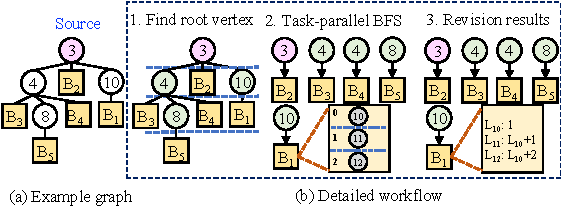
\includegraphics[width=1\linewidth]{figures/concurrent_bfs-crop.pdf}
%     \caption{Concurrent BFS on GIR using the BC tree structure. \YJ{Split "1. Find root nodes" to two lines. And then decrease the width of box 1.}}
%     \label{fig:concurrent_bfs}
% \end{figure}
% % \YJ{Maybe we should switch 6.1 and 6.2}

% % \YJ{Also, this is from my proposal writing.}

% We first illustrate the framework using breadth-first search (BFS), which is one of the most fundamental graph traversal algorithms and serves as the basis for many downstream analytics.
% % In AI supply chain analysis, traversal supports tasks such as \textit{dependency resolution} (e.g., ``what dataset does this model depend on?''), \textit{backward provenance tracing} (e.g., ``which models were influenced by a compromised dataset?''), and \textit{forward impact propagation} (e.g., ``how widely can a vulnerability in a shared dependency propagate?''). 
% We have built a hierarchical GIR. % which serves as a solid foundation for further graph analytics. 
% With that, we \textit{aim to design a scalable computation framework}.
% % As the queries often require quick responses, we would like to leverage the powerful computing hardware, e.g., Graphics Processing Units (GPUs).
% % \YJ{Why GPU?}
% % The AI supply chain graph is large-scale, heterogeneous, and dynamically evolving, encompassing millions of artifacts and dependencies across models, datasets, software, and hardware. Traditional CPU-based graph analytics struggle to scale due to irregular memory access patterns, fine-grained dependencies, and high update rates. 
% % While recent graph computing frameworks for GPUs--such as Gunrock, CuGraph, and Hornet--offer high throughput on static homogeneous graphs, they are not optimized for dynamic, semantically typed graphs with hierarchical structure such as our proposed GIR. 
% % This motivates the need for a novel GPU-accelerated computation framework tailored to GIR-level operations.
% % Our proposed computation framework is built around the GIR hierarchy defined in \underline{Task 2.1}. The GIR enables decomposition of the supply chain graph into WCCs, SCCs and BiCCs, offering natural macro-nodes that partition computation. Leveraging this structure, we design scalable, modular, and update-aware GPU-based algorithms for critical supply chain analytics tasks, including traversal, structure-aware scoring, and spectral methods. 

% % \YJ{Need to write in one of the following ways.
% % 1. Take the graph traversal as an example to explain our idea. Similary ideas can be applied to path finding and centrality computation.
% % 2. Propose a general three-level computation framework, apply them separately to graph traversal, path finding, and centrality.}

% % By expanding algorithmic coverage, we ensure that our GIR framework remains computationally versatile and capable of enabling advanced tasks such as compliance verification, risk modeling, and ecosystem evolution analysis.


% % In addition, during the course of this project, we would like to explore the support for many other graph algorithms, such as 
% % By exploiting GIR's structural decomposition and parallel-friendly properties, this thrust targets significant speedups in computation, paving the way for real-time and large-scale AI supply chain analytics on modern GPU hardware.


% % \textbf{Task 3.1: Structure-Aware Computation over the GIR}
% % The structural hierarchy of the GIR provides a natural platform for scalable graph computation. Standard graph queries--such as reachability, subgraph matching, provenance tracing, and vulnerability analysis--become more efficient when executed over macro-nodes rather than flat graphs. The research problem is to develop algorithms that leverage this structure while preserving semantic accuracy and performance guarantees.

% % We propose three classes of GIR-aware algorithms. First, we design hierarchical traversal methods that first query across the SCC-level DAG (e.g., ``which models are downstream of this dataset?''), then expand into the BiCCs as needed. This limits the search space and improves cache locality. Second, we develop AP/BiCC-based criticality scoring methods that identify vulnerable or high-impact artifacts by analyzing structural bottlenecks. For example, a dataset serving as an articulation point between two BiCCs may be a critical chokepoint. Third, we build propagation models for security risk and influence tracking that simulate cascading effects across the GIR. For example, if a vulnerable software library node is updated, we can quickly trace which models and datasets are indirectly dependent on it by traversing the GIR graph.

% % Each of these algorithms will be implemented in a modular fashion and benchmarked for time, space, and accuracy. We will evaluate their utility in case studies involving dependency tracking, license violation detection, and provenance reconstruction.

% % \noindent\textbf{Thrust 3: A GPU-Accelerated Computation Framework for GIR-based AI Supply Chain Analytics.} Building upon the hierarchical Graph Intermediate Representation (GIR) developed in Thrust 2, this thrust aims to develop a high-performance GPU-accelerated computation framework tailored to the unique demands of AI supply chain analysis. The GIR enables compact, modular organization of the graph structure, significantly reducing computational redundancy and data movement. 

% % \YJ{Connect the previous three types of algorithms with the following framework.}

% % These queries often require real-time responses over large-scale, dynamic graphs. 
% % However, existing GPU-based traversal frameworks such as Gunrock~\cite{wang2016gunrock}, CuGraph~\cite{team2019cugraph}, and GraphBLAST~\cite{yang2020graphblast} are optimized for monolithic graphs and do not natively support the hierarchical decomposition or structural indexing provided by our GIR.

% % \textbf{Proposed research.} 
% This task proposes to design a \textit{multi-step concurrent computation method} atop our GIR.
% % \textit{The goal is to design a practical and scalable framework for querying and analyzing evolving AI supply chain graphs.}
% % Particularly, 
% % which provides a hierarchical decomposition of the AI supply chain graph. 
% % This dramatically improves both task and data parallelism in a principled and structure-aware manner.

% \textbf{Multi-step computation on GIR.}
% Given a source vertex, computation proceeds in four stages.
% First, we traverse the SCC condensation DAG to prune the graph at the coarsest level.
% Because the DAG captures global dependencies among SCCs and is much smaller than the full graph, this step quickly identifies the reachable portion of the graph.
% Only SCCs reachable from the source SCC are retained for subsequent processing.
% This early pruning reduces the workload substantially, especially for traversal styles such as bottom-up BFS~\cite{beamer2012direction}, where the cost depends heavily on the number of remaining unexplored vertices.
% The time complexity of this stage is $\mathcal{O}(|V_{DAG}| + |E_{DAG}|)$.
% % \YJ{Time complexity, $\mathcal{O}(|V_{DAG}| + |E_{DAG}|$)}

% Second, within the retained region, we use the BC-tree structure to organize finer-grained execution.
% We conceptually unify the relevant BC trees and perform a traversal from the source to identify the entry/root node of each block.
% This step produces an execution plan in which each block becomes a natural computation unit.
% Its complexity is $\mathcal{O}(|V_T|)$, where $V_T$ denotes the vertices in the traversed tree structure.
% For the example in Figure~\ref{fig:concurrent_bfs}(a), the root of each block is determined by its parent in the BC tree.
% % , as the edge count is $|V_{BC}|-1$.
% % identify the root node for each block. 
% % This sets up an execution plan where each block's BFS can be executed independently in parallel.

% Third, we execute concurrent BFS over the selected blocks.
% Each block is treated as an independent task, enabling task parallelism across blocks; for example, each task may be assigned to a GPU cooperative thread array (CTA).
% Because blocks are largely independent once their entry points are known, this decomposition reduces communication and synchronization overhead.
% Within each block, we further apply conventional data-parallel BFS to compute local levels relative to the block root.
% The complexity of this stage is $\mathcal{O}(|V_s| + |E_s|)$, where $V_s$ and $E_s$ denote the vertices and edges in scope, respectively.
% In Figure~\ref{fig:concurrent_bfs}, five BFS tasks can be executed concurrently.
% % \YJ{Time complexity, $\mathcal{O}(|V_{s}| + |E_{s}|$)}

% Finally, we refine local results into global BFS levels.
% For each vertex, the final level is obtained by combining the absolute level of the block root with the relative level computed inside the block.
% As shown in Figure~\ref{fig:gir_bfs}(c), this refinement step reconciles levels across multiple blocks and restores a globally consistent traversal result.
% Its time complexity is $\mathcal{O}(|V_s|)$.
% % This ensures consistent levels across the entire graph. 

% Overall, the runtime is dominated by the third stage, since in practice $|V_s| \gg |V_T|$ and $|V_s| \gg |V_{DAG}|$.
% The advantage of our framework is therefore not in reducing the asymptotic cost of local traversal itself, but in exposing much more task parallelism than conventional flat-graph BFS, which mainly relies on data parallelism alone.
% Moreover, the same task decomposition can also be applied to DFS, suggesting a practical way to parallelize a traditionally sequential and difficult-to-parallelize graph primitive.

% % \YJ{The BFS level is not correct for the current method. It will be correct if we work on the BC+ tree.}
% % \YJ{Working on.}

% Same stradegy could be used when the edges have weight, then we can fully use this as SSSP.

% %\CQ{If a new SCC is formed, how could we quickly find it?
% %1. This only affects the vertices having the ranks between the source and target. 
% %2. FW-BW, color propagation. Bi-direction BFS, meet-in-the-middle
% %.}

% \textbf{Generalization to other graph analytics.}
% The same hierarchical principle extends naturally beyond BFS.
% In general, our framework supports three major classes of graph analytics: reachability, path finding, and centrality.
% The common pattern is to use GIR for hierarchical pruning at the top levels and concurrent execution at the lower levels.
% \CQ{common summarize} We use our framework to learvage the parallelism

% For \textit{reachability} and other unordered traversal tasks, GIR enables aggressive pruning before exploration begins.
% We first operate on the SCC condensation DAG and keep only the SCC supernodes that may lie on a valid traversal path.
% Within each retained SCC, we further use the BC tree structure to restrict exploration to the blocks that contain the source, target, or necessary articulation boundaries.
% Combined with direction-optimizing strategies such as top-down/bottom-up switching, this hierarchical pruning turns a global traversal problem into a much smaller localized one.

% For \textit{path finding}, including SSSP, $k$-shortest paths (KSP), and related dependency-chain analysis, we follow a similar workflow.
% We first traverse the condensation DAG to identify SCCs that may participate in the global path, then analyze the BC-tree structure inside those SCCs to determine relevant BiCC roots and block-level execution units.
% Each BiCC can then be processed as an independent task, which exposes both task-level and data-level parallelism.
% For example, we may apply $\Delta$-stepping for SSSP~\cite{meyer2003delta} and our prior PeeK algorithm for KSP~\cite{feng2023peek}, and then combine local results into global distances and paths.

% For \textit{centrality} computation, GIR is particularly beneficial because many centrality measures repeatedly solve shortest-path-like subproblems.
% Metrics such as betweenness centrality and closeness centrality are widely used to identify influential models, critical datasets, or vulnerable software dependencies in AI supply chain graphs~\cite{brandes2001faster,wang2016articulation}.
% By leveraging the BiCC structure and articulation points maintained in GIR, we can eliminate redundant shortest-path computations across articulation boundaries.
% In particular, we adopt the Articulation Points Guided Redundancy Elimination for Betweenness Centrality (AP-BC) method~\cite{wang2016articulation}, which aligns naturally with our hierarchy and further improves scalability.

% In summary, our hierarchical concurrent computation framework uses GIR not only as a structural representation, but also as an execution substrate.
% The condensation DAG supports coarse-grained pruning, the BC-tree exposes task-level decomposition, and local subgraphs enable data-parallel execution.
% Together, these levels provide a unified way to accelerate a broad class of dynamic graph analytics while preserving correctness and extensibility.